\section[Скоринговые системы]{СКОРИНГОВЫЕ СИСТЕМЫ}

\subsection{Описание предметной области}

\emph{Кредитный скоринг} --- система оценки кредитоспособности (кредитных рисков) лица,
основанная на численных статистических методах~\cite{wiki_credit_score}.

По сути, скоринг является методом классификации совокупности заемщиков на различные группы,
когда необходимая характеристика не известна, однако, известны другие характеристики,
которые каким-либо образом коррелируют с интересующей~\cite{rumyantsev2006}.
На практике, в зависимости от задач анализа заемщика, кредитный скоринг включает
\emph{application-скоринг} --- оценку кредитоспособности претендентов на получение кредита
(скоринг по анкетным данным используется в первую очередь),
\emph{behavioral-скоринг} --- оценка вероятности возврата выданных кредитов
(поведенческий анализ), а также
\emph{collection-скоринг} --- оценка возможности полного либо частичного возврата кредита
при нарушении сроков погашения задолженности (расчет рисков по портфелю).

\emph{Скоринговая система} представляет собой сложную систему автоматизации
выдачи потребительских кредитов в банковских отделениях, торговых точках, через интернет,
которая в качестве аналитического ядра использует решение одной из известных компаний-разработчиков.

Скоринговая система состоит из модуля подготовки исходных данных,
аналитического модуля и модуля отчетности.
Данные системы скоринга, могут быть трех типов.
Первый тип --- знания персонала кредитных отделов банков о конкретных типах кредитных
продуктов (потребительских, авто и ипотечного кредитования) и своих клиентах.
Второй тип данных --- статистика по уже выданным кредитам, учитывающая <<хороших>>
и <<плохих>> заемщиков. И, если банк не обладает ни одним из типов указанных данных ---
ни экспертными знаниями, ни статистикой выданных кредитов, модель,
лежащая в основе системы скоринга, преимущественно строится на основе региональных и отраслевых данных.

Все фронт-офисные решения для автоматизации процесса потребительского кредитования в большинстве случаев
представляют собой Web-приложения, что обеспечивает хорошую масштабируемость системы и
простоту подключения к процессу выдачи кредитов новых отделений банка и представительств в торговых точках.

\subsection{Обзор существующих решений}

Рассматривая различные скоринговые решения, корректно говорить о системах для западного рынка
и о системах для отечественного рынка, так как есть и западные поставщики,
например, EGAR, которые предлагают версию скоринга, полноценно учитывающую местную специфику.
Безусловно, системы для западного рынка значительно более функциональны,
чем разработки для СНГ, но заставить их работать в отечественных условиях трудно:
необходимо пройти сложный процесс внедрения, интеграции и адаптации~\cite{rumyantsev2006}.

Наиболее известными западными скоринговыми системами сегодня считаются
SAS Credit Scoring, SAP Credit Risk, EGAR Scoring, Transact SM (Experian-Scorex),
K4Loans (KXEN), Clementine (SPSS). Рассмотрим некоторые из них.

\subsubsection{SAP Кредитный риск}

Модуль <<SAP Кредитный риск>> содержит инфраструктуру, которая может использоваться
для вычисления показателей размера риска, таких как размер риска во взыскании и достаточность капитала.
Посредством метода калькуляции и установок, которые выполняются в пользовательской настройке,
производится управление пределами, используемыми системой при вычислении показателей~\cite{sap_credit_risk}.

\begin{figure}[h!]
  \centering
  \fcolorbox{gray}{white}{
    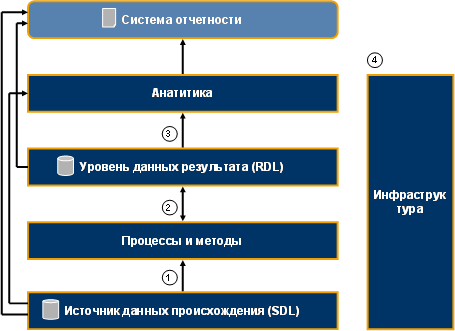
\includegraphics[width=100mm]{fig/sap_structure}
  }
  \caption{Структура модуля <<SAP Анализатор банка>>}
  \label{fig:sap_structure}
\end{figure}

Данный модуль является составной частью модуля <<SAP Анализатор банка>>,
имеющего структуру, представленную на рисунке~\ref{fig:sap_structure}.
Вместо непосредственного обмена информацией с модулем <<Кредитный риск>>
или использования предшествующих общих методов калькуляции и оценки эти исходные
системы сначала сохраняют данные на уровне исходных данных (SDL).
Модуль <<Кредитный риск>> может получить доступ к тем основным и переменным данным и переменные данным в SDL,
которые были предоставлены одной из исходных систем или первоначально созданы в SDL.
В модуле <<Кредитный риск>> можно использовать результаты, созданные предшествующими
общими методами калькуляции и оценки. Данные доступны с использованием уровня данных результатов (RDL)
или базы данных результатов (RDB),
поскольку именно в этих объектах хранятся данные результатов из модуля <<Общие методы калькуляции и оценки>>.

Результаты, вычисленные в модуле <<Кредитный риск>>, сохраняются также на уровне данных результатов
или в базе данных результатов. Место сохранения результатов определяется отдельно для каждого манданта.

\subsubsection{SAS Credit Scoring for Banking}

Инструментарий SAS Credit Scoring for Banking позволяет специалисту в области интеллектуального анализа
данных создавать модели кредитного скоринга для потребительских кредитов, кредитных карт, овердрафтов,
автомобильных, ипотечных и других кредитных продуктов.
Скоринг направлен на решение различных задач от оценки вероятности дефолта клиента до определения
стратегии работы коллекторского подразделения и создания рейтинговой системы в соответствии
с рекомендациями Базельского комитета~\cite{sas_scoring_for_banking}.

Основные общепринятые модели делятся на следующие типы, каждый из которых может быть реализован средствами
SAS Credit Scoring for Banking:
\begin{itemize}
\item анкетный (заявочный) скоринг;
\item поведенческий скоринг;
\item коллекторский скоринг;
\item антимошеннический скоринг;
\item модели PD, LGD, CCF/EAD в соответствии с Advanced-IRB подходом Базельского комитета.
\end{itemize}

Для анализа данных и разработки моделей SAS Credit Scoring for Banking предлагает своим пользователям
простой в использовании, но одновременно весьма гибкий и многофункциональный инструмент ---
SAS Enterprise Miner. SAS Enterprise Miner обладает интуитивно понятным графическим интерфейсом для
создания проектов по data mining и моделированию, представленным на рисунке~\ref{fig:sas_miner}.

\begin{figure}[h!]
  \centering
  \fcolorbox{gray}{white}{
    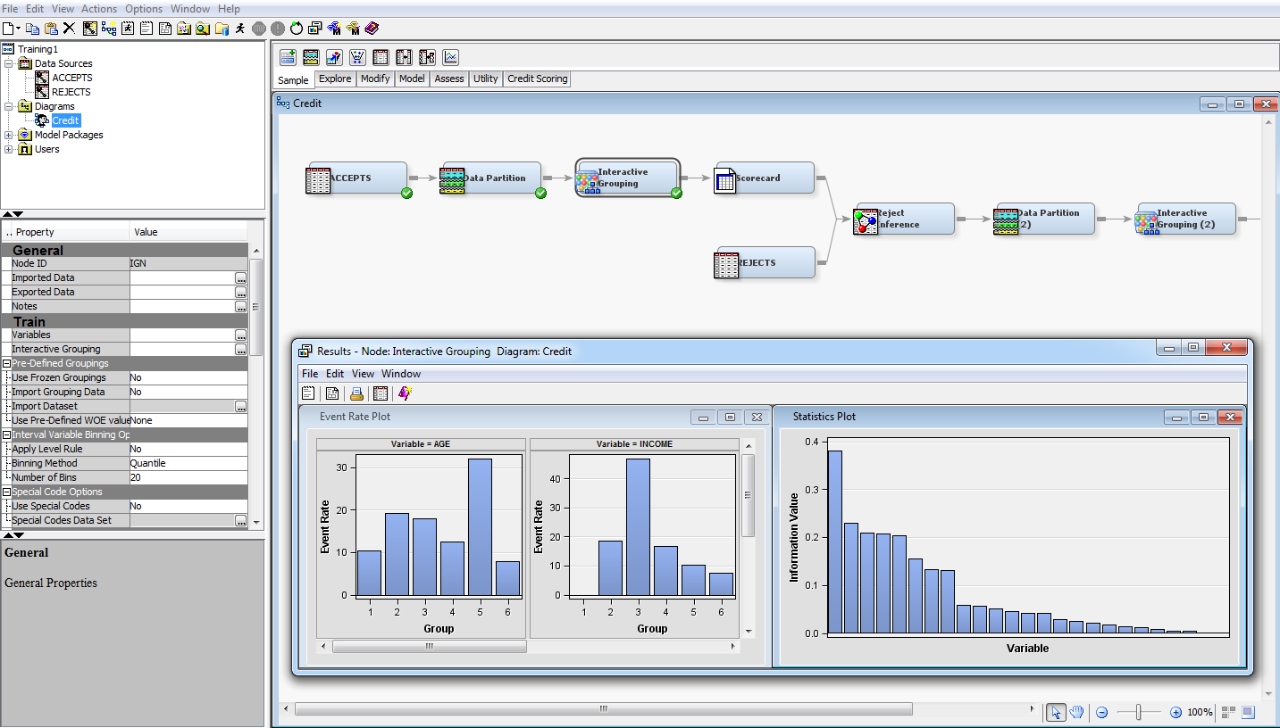
\includegraphics[width=100mm]{fig/sas_miner}
  }
  \caption{Пользовательский интерфейс приложения \\ <<SAS Enterprise Miner>>}
  \label{fig:sas_miner}
\end{figure}

Пользователям данной системы доступен широкий набор предустановленных отчетов валидации,
автоматически обновляемых на регулярной основе. Для упрощения работы с отчетами,
все ключевые показатели имеют настраиваемые цветовые индикаторы,
показывающие насколько хорошо пройден тот или иной тест, как показано на рисунке~\ref{fig:sas_tests}.

\begin{figure}[h!]
  \centering
  \fcolorbox{gray}{white}{
    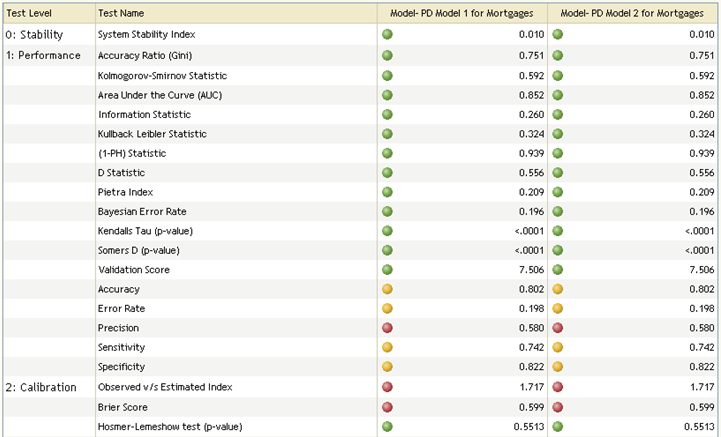
\includegraphics[width=100mm]{fig/sas_tests}
  }
  \caption{Пример отчета, сгенерированного приложением \\ <<SAS Сredit Scoring for Banking>>}
  \label{fig:sas_tests}
\end{figure}

Несмотря на то, что предустановленные отчеты уже содержат полноценную информацию о состоянии модели,
пользователь имеет возможность добавления отчетов и расчета собственных статистик.

Каждый отчет содержит значения соответствующих статистик, цветовые индикаторы и настраиваемый набор графиков,
отображая как статические значения параметров, так и динамику их изменения.
Кроме того, SAS Credit Scoring for Banking позволяет проводить валидацию не только на всем портфеле,
но и на любом его подсегменте при помощи задания бизнес-фильтров.
Тем самым аналитик имеет возможность не только выявлять сильные и слабые стороны модели,
но и изучать те сегменты клиентов, для которых она нуждается в корректировке.

\subsubsection{EGAR Scoring}

EGAR Scoring --- система оценки кредитоспособности потенциальных заемщиков ---
физических лиц и индивидуальных предпринимателей по информации,
указанной ими в заявлениях на получение кредита на основе анализа
исторических данных и применения современных макроэкономических моделей~\cite{egar_scoring}.
Система применяется в процессе андеррайтинга заёмщиков по потребительским кредитам,
кредитным картам, автокредитованию, ипотеке и кредитам малому бизнесу.
По результатам скоринга формируются отчеты с обоснованием принятого
решения о кредитоспособности.
Системой поддерживаются функции
скоринга по анкетным данным (EGAR Application Scoring),
поведенческий анализ (EGAR Behavior Scoring),
расчет рисков по портфелю (EGAR Collection Scoring).

Данная система является составной частью системы EGAR E4 Banking
по сквозной автоматизации операций банка в области кредитования физических лиц
и индивидуальных предпринимателей,
полностью покрывающей операции фронт- и бэк-офисов кредитной организации,
включая модули по обработке кредитной заявки, скорингу, учету кредитных договоров,
управлению резервом и задолженностью, управленческому учету для продуктов,
резервов и групп рисков, а также бухгалтерскому учету в стандартах РФ.
EGAR E4 Banking формирует четкие критерии определения кредитоспособности
заемщиков с использованием современных скоринговых и макроэкономических подходов.
К числу поддерживаемых типов продуктов относятся: целевой кредит, кредит на неотложные нужды,
кредиты под залог покупаемого имущества (авто- и ипотека)
и возобновляемые кредитные линии (кредитные карточки, овердрафт),
как показано на рисунке~\ref{fig:egar_structure}.

\begin{figure}[h!]
  \centering
  \fcolorbox{gray}{white}{
    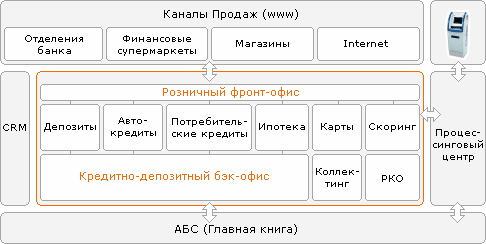
\includegraphics[width=100mm]{fig/egar_structure}
  }
  \caption{Функциональная схема пакета \\ <<EGAR E4 Banking>>}
  \label{fig:egar_structure}
\end{figure}

Технологическая платформа EGAR E4 Banking реализована в стандартах J2EE
c использованием преимуществ SOA-архитектуры.
Решение построено на концепции тонкого клиента и централизованного хранилища данных
и обладает широкими интеграционными возможностями.
Масштабирование системы достигается простым наращиванием централизованных
серверных ресурсов без изменения состава ПО в точках развертывания
при минимальном участии IT-специалистов.